% =====================================================================
%  CS 6330 - Introduction to Data Science
%  Homework 2: Data and Distributions
%  Author: Taek Lim
%
%  Build:  latexmk -pdf hw2_taeklim_report.tex
%      or: pdflatex hw2_taeklim_report.tex   (run twice for references)
%
%  Figure paths are relative to this file: ../figures/*.png
%  Figures and every number below come from ../code/p1.py and ../code/p2.py
%  (run from the repo root: uv run python hw2/code/p1.py).
% =====================================================================
\documentclass[11pt]{article}

\usepackage[letterpaper,margin=0.75in]{geometry}
\usepackage[T1]{fontenc}
\usepackage[utf8]{inputenc}
\usepackage{amsmath}
\usepackage{array}        % >{...} column modifiers
\usepackage{booktabs}     % \toprule \midrule \bottomrule
\usepackage{float}        % [H] = put the float exactly here, no deferring
\usepackage{graphicx}
\usepackage{caption}
\usepackage{listings}
\usepackage{xcolor}
\usepackage[hidelinks]{hyperref}

\lstset{
  basicstyle=\ttfamily\footnotesize,
  breaklines=true,
  frame=single,
  rulecolor=\color{gray!40},
  backgroundcolor=\color{gray!5},
  showstringspaces=false,
  columns=fullflexible,
  literate={α}{{$\alpha$}}1 {λ}{{$\lambda$}}1 {μ}{{$\mu$}}1 {σ}{{$\sigma$}}1
           {≥}{{$\geq$}}1 {≤}{{$\leq$}}1,
}

\captionsetup{font=small, labelfont=bf}

% Question heads: sky blue, bold. Darkened from a literal "sky blue" so the
% heading still reads on paper and in greyscale print.
\definecolor{headblue}{HTML}{0C6FB8}
\newcommand{\question}[2]{%
  \section*{\color{headblue}#1 \hfill \normalfont\small(#2)}}

% One model-vs-data figure: \modelfig{file}{caption}
\newcommand{\modelfig}[2]{%
  \begin{figure}[H]\centering
    \includegraphics[width=\linewidth]{../figures/#1.png}
    \caption{#2}
  \end{figure}}


\title{\textbf{Homework 2: Data and Distributions}\\[2pt]
       \large Fitting power-law, exponential, uniform and normal models}
\author{Taek Lim \\ \small CS 6330: Introduction to Data Science}
\date{\today}

\begin{document}
\maketitle

\noindent
\textbf{Data.} \texttt{airport\_routes.csv} (3409 airports, Feb 2017),
\texttt{movie\_votes.csv} (4392 TMDb average ratings),
\texttt{DoB.txt} (460{,}718 IMDb birth dates).\\
\textbf{Tooling.} Python 3 / pandas / numpy / scipy / matplotlib; all estimates
computed programmatically, none typed by hand; analysis code, figure code and write-up
drafted with Claude Code. Code is in Appendix~\ref{app:code} and in \texttt{hw2/code/}.

\vspace{1em}\hrule\vspace{1em}

% =====================================================================
\question{Problem 1: Fit four distributions to two datasets}{90 pts}

% Per the spec, parts (a)-(d) are repeated for EACH dataset:
%   (a) power law   -> alpha        (5 pts x 2 datasets)
%   (b) exponential -> lambda       (5 pts x 2)
%   (c) uniform     -> [a, b]       (5 pts x 2)
%   (d) normal      -> mu, sigma    (5 pts x 2)
% then, per dataset: distribution of the data (5 pts x 2) and the comparison
% against samples drawn from each fitted model + discussion (20 pts x 2).
% PDF, CDF or QQ plot -- one of the three is enough to support the conclusion.

\subsection*{Method}

Every parameter is the maximum-likelihood estimate for its model, computed from all
$n$ data points $x_1,\dots,x_n$:
\begin{align*}
  \text{power law:}   &\quad \hat\alpha = 1 + n\Big/\textstyle\sum_{i}\ln(x_i/x_{\min}),
                        \quad x_{\min} = \min_i x_i \\
  \text{exponential:} &\quad \hat\lambda = 1/\bar x \\
  \text{uniform:}     &\quad [\hat a, \hat b] = [\min_i x_i,\ \max_i x_i] \\
  \text{normal:}      &\quad \hat\mu = \bar x, \quad \hat\sigma = \text{sample standard deviation } (n-1)
\end{align*}
For each fitted model I drew $n$ random values (seed 6330) and compared them with the
data. Every comparison figure has two panels. The left panel overlays the data and the
model sample, as a CCDF on log-log axes for airports and as a PDF for movies. The right
panel is a QQ plot of the model-sample quantiles against the data quantiles, where
points on the dashed line $y = x$ mean the model reproduces the data. As one number per
model I also report the two-sample Kolmogorov--Smirnov distance $D$ (the largest gap
between the two CDFs; $0$ means identical and $1$ means no overlap).

% ---------------------------------------------------------------------
\subsection*{Dataset A: airport routes}

\subsubsection*{(a) Power law: $\alpha$}
$\hat\alpha = 1.612$, with $x_{\min} = 1$ route.

\subsubsection*{(b) Exponential: $\lambda$}
$\hat\lambda = 1/19.845 = 0.0504$ (mean 19.85 routes).

\subsubsection*{(c) Uniform: $[a, b]$}
$[a, b] = [1, 915]$.

\subsubsection*{(d) Normal: $\mu$ and $\sigma$}
$\hat\mu = 19.845$, $\hat\sigma = 53.506$.

\subsubsection*{Distribution of the data}

\begin{figure}[H]\centering
  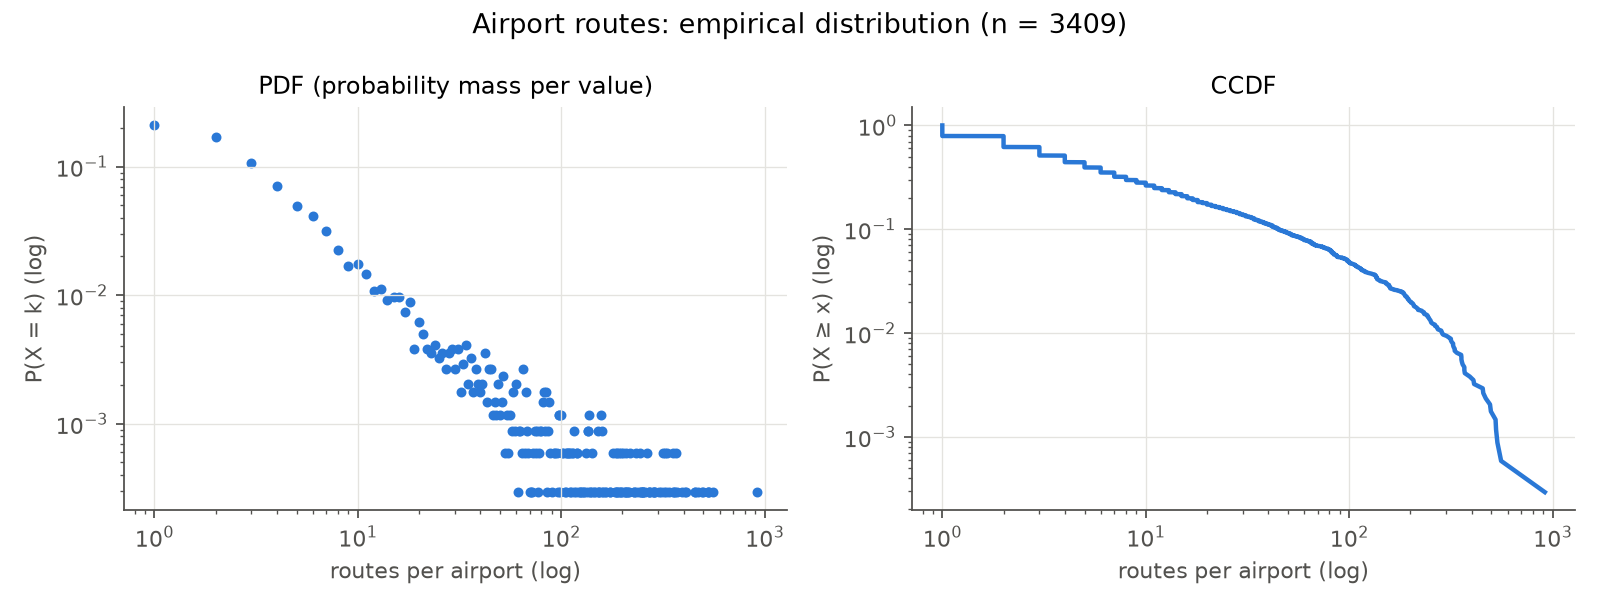
\includegraphics[width=\linewidth]{../figures/p1a_0_data.png}
  \caption{Airport routes. Left: share of airports with exactly $k$ routes. Right:
  share with at least $x$ routes. Both are on log-log axes. The median airport has 4
  routes and 38\% have only 1 or 2, while the busiest has 915. The mean (19.8) is five
  times the median and the skewness is 6.0, so a few hubs hold most of the routes.}
\end{figure}

\subsubsection*{The data compared with each fitted model}

\modelfig{p1a_1_powerlaw}{If the data were a power law ($\alpha = 1.612$, $x_{\min} = 1$).
  The CCDF follows the data from 1 to about 60 routes, and the QQ points lie on
  $y = x$ over that range. Above about 100 routes the model keeps going and produces
  airports with $10^4$ to $10^5$ routes, while the data bends down and stops at 915.
  KS $D = 0.209$.}

\modelfig{p1a_2_exponential}{If the data were exponential ($\lambda = 0.0504$). The
  model has too few small airports (its sample goes below 1 route, which the data never
  does) and a tail that dies out at about 150 routes. The QQ points are too flat: the model
  overstates small airports and understates hubs. KS $D = 0.379$.}

\modelfig{p1a_3_uniform}{If the data were uniform on $[1, 915]$. A typical sampled airport
  has about 460 routes, but 99\% of real airports have fewer than 285. The CCDF of the
  model stays near 1 until the right edge, and the QQ points lie far above $y = x$ for
  every quantile. KS $D = 0.857$, the worst of the four.}

\modelfig{p1a_4_normal}{If the data were normal ($\mu = 19.8$, $\sigma = 53.5$). With
  $\sigma$ almost three times $\mu$, 36\% of the model's mass is below zero, which is
  impossible for a route count. The log axes can only show the positive part. The model's
  tail is also thin and ends near 200 routes. KS $D = 0.358$.}

\subsubsection*{Which model fits, and why}

\begin{center}
\begin{tabular}{lcccc}
  \toprule
  & power law & exponential & uniform & normal \\
  \midrule
  KS distance $D$ (data vs model sample) & \textbf{0.209} & 0.379 & 0.857 & 0.358 \\
  \bottomrule
\end{tabular}
\end{center}

\noindent
\textbf{The airport data follows a power law, with a cutoff in the far tail.}
It is the only one of the four models whose CCDF is a straight line on log-log axes. The
data's CCDF is close to straight for more than two decades (1 to about 100 routes), and
the power-law sample matches it there. The other three models fail for structural
reasons, not because a parameter is slightly off:
\begin{itemize}
  \item \textbf{Uniform} says every route count from 1 to 915 is equally likely, but most
        airports are tiny.
  \item \textbf{Normal} is symmetric and allows negative counts, while the data is
        bounded below at 1 and skewed to the right (skewness 6.0).
  \item \textbf{Exponential} has the right shape (many small, few large), but its tail
        falls off too fast. With $\lambda = 0.05$, an airport with 500 routes has
        probability about $e^{-25}$, yet the data has five airports with more than 500.
\end{itemize}
The power law is not a perfect fit. $\hat\alpha = 1.61$ is below 2, so the fitted model
has an infinite mean and its samples contain airports with $10^5$ routes. Real
airports cannot grow that large: there are only 3409 airports to fly to, and runways,
gates and slots limit the busiest hubs. That is why the data's CCDF bends down above
about 100 routes. The best description is a power law with an upper cutoff, which is
typical of networks that grow by preferential attachment: new routes go
mostly to airports that already have many routes.

% ---------------------------------------------------------------------
\clearpage
\subsection*{Dataset B: movie votes}

\subsubsection*{(a) Power law: $\alpha$}
$\hat\alpha = 1.851$, with $x_{\min} = 1.9$ (the lowest average vote).

\subsubsection*{(b) Exponential: $\lambda$}
$\hat\lambda = 1/6.227 = 0.1606$ (mean vote 6.23).

\subsubsection*{(c) Uniform: $[a, b]$}
$[a, b] = [1.9, 8.5]$.

\subsubsection*{(d) Normal: $\mu$ and $\sigma$}
$\hat\mu = 6.227$, $\hat\sigma = 0.893$.

\subsubsection*{Distribution of the data}

\begin{figure}[H]\centering
  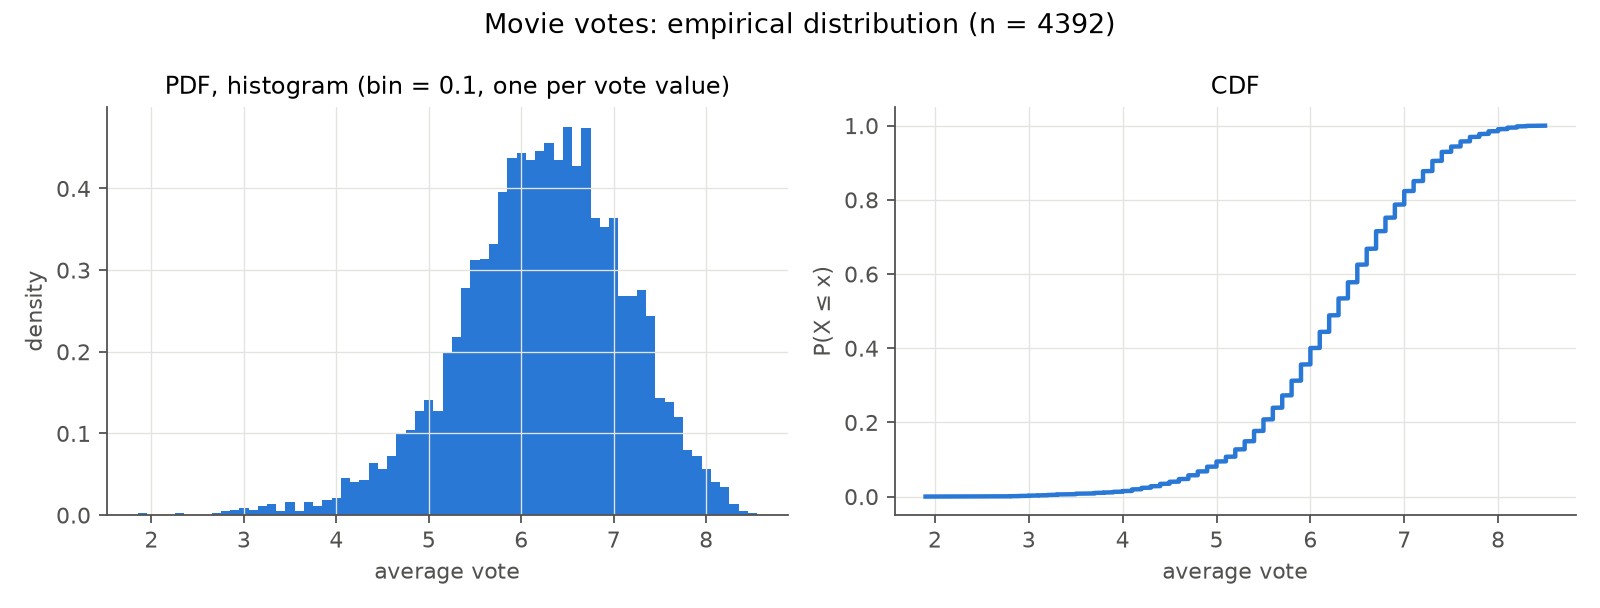
\includegraphics[width=\linewidth]{../figures/p1b_0_data.png}
  \caption{Movie votes. Left: histogram with one bin per possible vote (votes are
  rounded to 0.1). Right: empirical CDF. The distribution has one peak and is nearly
  symmetric around 6.3 (median 6.3, mean 6.23). The left tail is somewhat longer
  (skewness $-0.48$): a few movies are rated 2 to 4, and none are above 8.5.}
\end{figure}

\subsubsection*{The data compared with each fitted model}

\modelfig{p1b_1_powerlaw}{If the data were a power law ($\alpha = 1.851$, $x_{\min} = 1.9$).
  The model puts its highest density at the lowest vote, which is where the data has
  almost nothing, and 13\% of its sample lies above 20, which is not a possible rating.
  The QQ plot is on log axes because the sample goes up to about 1000.
  KS $D = 0.485$.}

\modelfig{p1b_2_exponential}{If the data were exponential ($\lambda = 0.1606$). The model
  also peaks at zero and has a long right tail (4\% of its sample is above 20). In the QQ
  plot the points cross $y = x$ at a steep angle, so the model's spread is far larger
  than the data's. KS $D = 0.490$.}

\modelfig{p1b_3_uniform}{If the data were uniform on $[1.9, 8.5]$. The model is flat, but
  the data is concentrated between 5 and 7.5. The QQ plot is an S-shape: the model's
  low quantiles are too low and its high quantiles too high. KS $D = 0.394$.}

\modelfig{p1b_4_normal}{If the data were normal ($\mu = 6.227$, $\sigma = 0.893$). The
  sample traces the same bell as the data, and the QQ points lie on $y = x$ from about
  4.5 to 7.5. The only departures are at the ends: the data's lowest votes are lower
  than the model predicts (longer left tail), and the data stops at 8.5 while the model
  continues. KS $D = 0.055$, by far the smallest.}

\subsubsection*{Which model fits, and why}

\begin{center}
\begin{tabular}{lcccc}
  \toprule
  & power law & exponential & uniform & normal \\
  \midrule
  KS distance $D$ (data vs model sample) & 0.485 & 0.490 & 0.394 & \textbf{0.055} \\
  \bottomrule
\end{tabular}
\end{center}

\noindent
\textbf{The movie votes follow a normal distribution, approximately.}
The data has one peak near the middle of its range and is close to symmetric. The
normal model predicts 68.3\% of movies within $\pm1\sigma$ and 95.4\% within
$\pm2\sigma$; the data has 70.1\% and 95.6\%. In the QQ plot the points lie on the
identity line through the bulk of the data, and the KS distance is about one seventh of
the next-best model's.

The other three models fail for structural reasons. The power law and the exponential
are both monotonically decreasing: their most likely value is the smallest one, so they
predict mostly terrible movies and a long tail of ratings above 10. The uniform model
ignores the peak altogether.

The fit is good but not exact, for two reasons. First, the data is bounded to $[1, 10]$
and slightly left-skewed: bad movies can drop further below the average than good movies
can rise above it. Second, votes are rounded to one decimal, which gives the QQ plot its
small steps. A normal shape is expected because each value is an \emph{average} of many
individual votes. By the central limit theorem an average of many independent ratings
tends toward a normal distribution, whatever the distribution of each single rating.

% =====================================================================
\clearpage
\question{Problem 2: Age, first digit and last digit}{30 pts}

% NOTE: the spec says FIRST digit and LAST digit (hw2_introduction.txt says
% "smallest/largest" -- the PDF wins). For age 34: first = 3, last = 4.

\subsection*{Computing the ages}

The birth dates have the form \texttt{dd-Mon-yy} (a few use a 4-digit year). I read
every 2-digit year as 19\textit{yy}. IMDB-WIKI was collected in 2015, so a year such as
\texttt{20}--\texttt{24} cannot mean 2020--2024. Also, the counts per year decrease
smoothly from the 1920s down to \texttt{00}, with no break that would mark a switch to
the 2000s. The 129 rows with year \texttt{0000} (a missing-value placeholder) were
dropped. Age is the number of completed years on 2015-01-01, the dataset's collection
year. Keeping ages 1 to 99 leaves \textbf{458{,}015} people (mean 45.3, median 43,
range 15 to 99). The minimum of 15 is a result of the 19\textit{yy} rule, since the latest
possible birth year is 1999.

\subsection*{Distribution of age}

\begin{figure}[H]\centering
  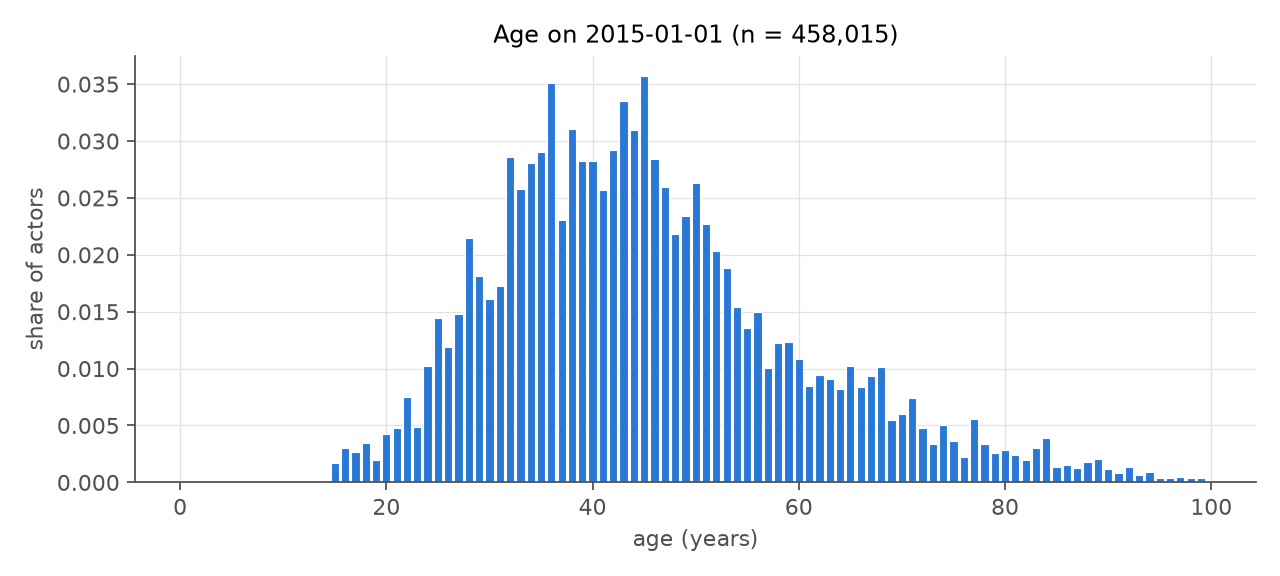
\includegraphics[width=0.9\linewidth]{../figures/p2_1_age.png}
  \caption{Age in 2015. The distribution has one broad peak in the 30s and 40s and a long right
  tail up to 99. Most of the mass is between 25 and 60. No age is below 15, but that comes
  from the parsing rule: with every 2-digit year read as 19\textit{yy}, the latest possible
  birth year is 1999.}
\end{figure}

\subsection*{Distribution of the first digit}

\begin{figure}[H]\centering
  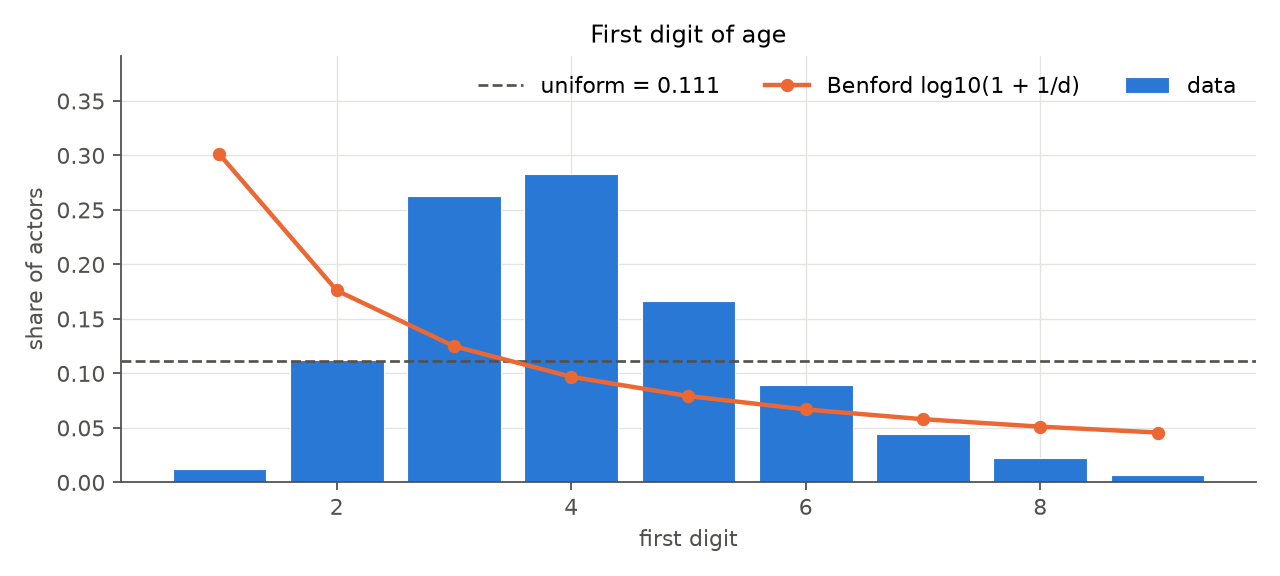
\includegraphics[width=0.9\linewidth]{../figures/p2_2_first_digit.png}
  \caption{First digit of age, with the uniform level $1/9$ (dashed) and Benford's law
  (orange). The shares are 1.3\%, 11.3\%, 26.2\%, 28.3\%, 16.7\%, 9.0\%, 4.4\%, 2.2\% and
  0.7\% for digits 1 to 9. The data is far from uniform and also far from Benford: it
  peaks at 3 and 4, where Benford predicts a steady decline from 1.}
\end{figure}

\subsection*{Distribution of the last digit}

\begin{figure}[H]\centering
  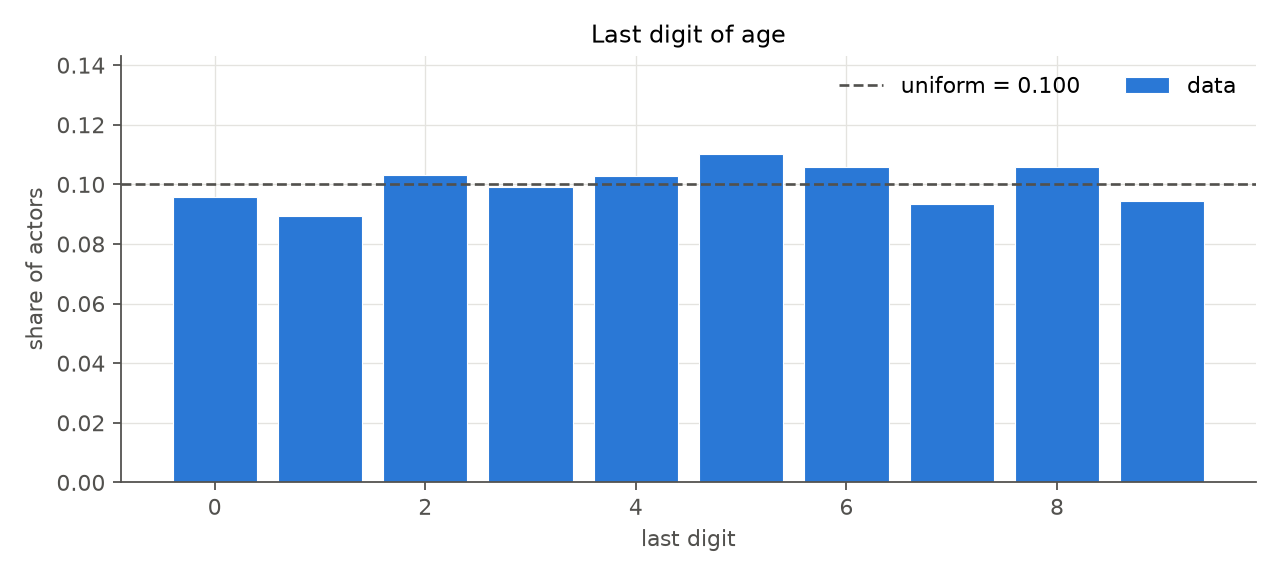
\includegraphics[width=0.9\linewidth]{../figures/p2_3_last_digit.png}
  \caption{Last digit of age, with the uniform level $1/10$ (dashed). Every digit has a
  share between 8.95\% and 11.01\%, within 1.1 percentage points of 10\%.}
\end{figure}

\subsection*{Discussion: which digits are uniform, and why}

\textbf{The last digit is uniform (approximately); the first digit is not.}

\paragraph{Last digit.} This is expected. The last digit of an age is its value modulo
10. Every block of ten ages (20--29, 30--39, \dots) contains each last digit exactly
once. The age distribution changes slowly compared with a step of one year, so within
any block of ten the ten ages have roughly equal counts, and summing over the blocks
gives each last digit about 10\%. The remaining deviations of up to $\pm1.1$ points come
from year-to-year noise in how many actors were born in a given year (the jagged bars in
the age histogram), not from any preference for particular digits.

\paragraph{First digit.} This is also expected once you notice that, for ages 10 to
99, the first digit \emph{is} the decade of life. Its histogram is therefore the age
distribution grouped by decade, and it has the same shape as the age distribution: one
peak (in the 30s and 40s) with a right tail. Digit 1 is almost empty because only ages
15 to 19 are possible and few actors are that young, and 9 is almost empty because few
actors reach their 90s. For the first digit to be uniform, every decade from teens to 90s would need
the same number of actors, which working actors clearly are not.

\paragraph{It is not Benford's law either.} Benford's law (first digit $d$ with
probability $\log_{10}(1 + 1/d)$, so 1 is the most common at 30.1\%) applies to data
that spans several orders of magnitude, such as populations, prices or the airport
route counts in Problem~1, where the log of the value is spread out roughly evenly.
Age spans less than one order of magnitude (15 to 99) and is concentrated around 45, so
its first digit shows where that one hump sits, not Benford's pattern. In short, the
last digit is uniform because it throws away where the value is and keeps only its
position within a block of ten. The first digit keeps exactly that information, so its
distribution follows the shape of the age distribution.

% =====================================================================
\clearpage
\appendix
\section{Code}\label{app:code}

\subsection*{Problem 1: \texttt{hw2/code/p1.py}}
\lstinputlisting[language=Python]{../code/p1.py}

\subsection*{Problem 2: \texttt{hw2/code/p2.py}}
\lstinputlisting[language=Python]{../code/p2.py}

\end{document}
